%-----------------------------------LICENSE------------------------------------%
%   This file is part of tikz_figures.                                         %
%                                                                              %
%   tikz_figures is free software: you can redistribute it and/or              %
%   modify it it under the terms of the GNU General Public License as          %
%   published by the Free Software Foundation, either version 3 of the         %
%   License, or (at your option) any later version.                            %
%                                                                              %
%   tikz_figures is distributed in the hope that it will be useful,            %
%   but WITHOUT ANY WARRANTY; without even the implied warranty of             %
%   MERCHANTABILITY or FITNESS FOR A PARTICULAR PURPOSE.  See the              %
%   GNU General Public License for more details.                               %
%                                                                              %
%   You should have received a copy of the GNU General Public License along    %
%   with tikz_figures.  If not, see <https://www.gnu.org/licenses/>.           %
%------------------------------------------------------------------------------%

% Use the standalone class for displaying the tikz image on a small PDF.
\documentclass[crop, tikz]{standalone}

% Import the tikz package to use for the drawing.
\usepackage{tikz}

% The arrows package is used for the LaTeX arrow.
\usetikzlibrary{arrows.meta}

% Begin the document.
\begin{document}

    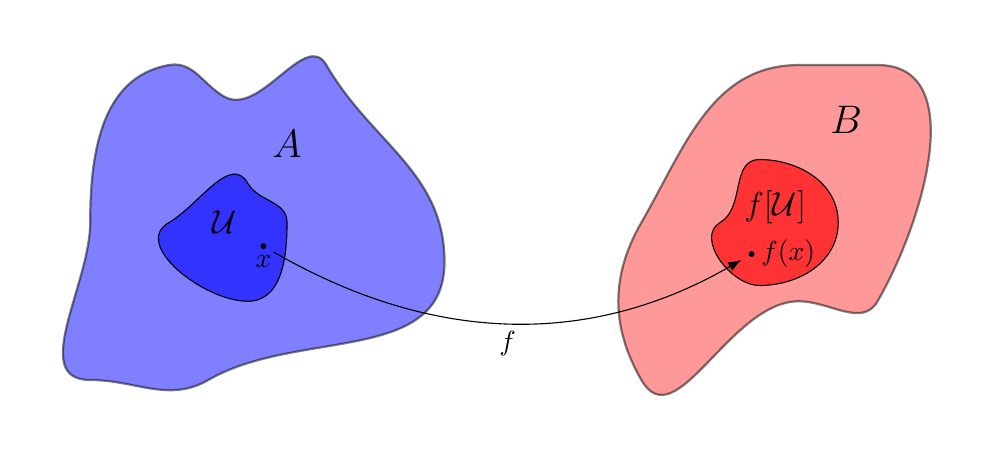
\begin{tikzpicture}[>=Latex]
        \coordinate (U1) at (-5.0, -2.0);
        \coordinate (U2) at (-3.5, -2.0);
        \coordinate (U3) at (-0.5, -0.5);
        \coordinate (U4) at (-2.0,  2.0);
        \coordinate (U5) at (-3.3,  1.6);
        \coordinate (U6) at (-4.0,  2.0);
        \coordinate (U7) at (-5.0,  0.0);

        \coordinate (V1) at (5.0,  2.0);
        \coordinate (V2) at (4.0,  2.0);
        \coordinate (V3) at (2.0,  0.0);
        \coordinate (V4) at (2.0, -2.0);
        \coordinate (V5) at (4.0, -1.0);
        \coordinate (V6) at (5.0, -1.0);

        \coordinate (S1) at (-4.0,  0.0);
        \coordinate (S2) at (-3.0, -1.0);
        \coordinate (S3) at (-2.5,  0.0);
        \coordinate (S4) at (-3.0,  0.5);

        \coordinate (T1) at (3.0,  0.0);
        \coordinate (T2) at (3.5, -0.8);
        \coordinate (T3) at (4.5,  0.0);
        \coordinate (T4) at (3.5,  0.8);

        \coordinate (x)  at (-2.8, -0.3);
        \coordinate (fx) at (3.4,  -0.4);

        \draw[fill=blue,opacity=0.5,draw=black,thick]
            (U1)    to[out=0,  in=-150] (U2)
                    to[out=30, in=-90]  (U3)
                    to[out=90, in=-60]  (U4)
                    to[out=120, in=-30] (U5)
                    to[out=150,in=10]   (U6)
                    to[out=-170,in=90]  (U7)
                    to[out=-90,in=180]  cycle;

        \draw[fill=red!80!white,opacity=0.5,draw=black,thick]
            (V1)    to[out=180, in=0]       (V2)
                    to[out=180, in=60]      (V3)
                    to[out=-120,in=120]     (V4)
                    to[out=-60, in=180]     (V5)
                    to[out=0,   in=-120]    (V6)
                    to[out=60,  in=0]       cycle;

        \draw[fill=blue!80!white] (S1)  to[out=-150,in=180] (S2)
                                        to[out=0,   in=-90] (S3)
                                        to[out=90,  in=-60] (S4)
                                        to[out=120, in=30]  cycle;

        \draw[fill=red!80!white] (T1)   to[out=-150,in=180] (T2)
                                        to[out=0,   in=-90] (T3)
                                        to[out=90,  in=0]   (T4)
                                        to[out=180, in=30]  cycle;

        \draw[fill=black] (x)  circle (0.3mm);
        \draw[fill=black] (fx) circle (0.3mm);
        \node at (-2.5, 1.0) {\Large{$A$}};
        \node at ( 4.6, 1.3) {\Large{$B$}};
        \node at (-3.3, 0.0) {\large{$\mathcal{U}$}};
        \node at ( 3.7, 0.2) {\large{$f[\mathcal{U}]$}};
        \node at (x)  [below] {$x$};
        \node at (fx) [right] {$f(x)$};
        \draw[->,shorten >= 1.5mm,shorten <= 1.5mm]
            (x) to[out=-30,in=-150] node[below]{$f$} (fx);
    \end{tikzpicture}

\end{document}